Przedmiotem pracy jest stworzenie prototypowego serwera oraz klienta HTML5. Zadaniem serwera jest jest udostępnienie usługi uruchamiającej aplikacje oparte o biblioteki \emph{Qt} i KDE. Zdalny dostęp do aplikacji uruchomionej w środowisku serwera jest dostępny poprzez interfejs HTML5 udostępniany przez instancję serwera.

Użytkownik serwisu w celu skorzystania z aplikacji \emph{Qt} zainstalowanej na serwerze wchodzi na odpowiedni adres przy użyciu nowoczesnej przeglądarki internetowej. Następnie wybiera interesujący go program i przejmuje nad nim kontrolę. Jest w stanie wyświetlić program w przeglądarce, który wizualnie odpowiada rzeczywistej instancji uruchomionej na serwerze. Wszystkie akcje myszy oraz klawiatury przechwycone przez przeglądarke są wysyłane do serwera, dzięki czemu użytkownik ma pełną kontrolę nad uruchomioną aplikacją. Należy również zaimplementować odpowiednik menedżera okien (ang. window manager) po stronie klienta, aby udostępnić użytkownikowi funkcjonalność pracy z wieloma oknami --- przesuwanie, rozszerzanie, zamykanie, oraz opcjonalnie minimalizowanie oraz maksymalizowanie.

// TODO: Wymagania (ogólne)
// TODO: Przypadki użycia
// TODO: Zachowanie systemu / software'u
// TODO: Struktura systemu / software'u

Postawione zadanie w głównej mierze polega na rozwiązaniu czterech podstawowych problemów:
\begin{enumerate}
  \item komunikacja między klientem a serwerem,
  \item komunikacja między klientem a aplikacją,
  \item uzyskanie informacji o wyglądzie elementów graficznego interfejsu aplikacji,
  \item symulacja interakcji użytkownika z interfejsem aplikacji.
\end{enumerate}

Na rysunku \ref{fig:arch} przedstawiono ideowy schemat architektury systemu rozwiązującego powyższe kwestie. 
Podstawą projektu jest jego modułowość, która separuje logikę odpowiedzialną za udostępnianie interfejsu WWW inicjującego proces aplikacji Qt od części stanowiącej węzeł komunikacyjny pomiędzy klientem a aplikacją Qt działąjącą po stronie serwera.
Można również zauważyć bardzo wyraźne rozgraniczenie między dwoma kanałami przesyłu danych, które wynika z konieczności umożliwienia korzystania z serwera wielu klientom. 
W dalszej części przedstawiono opisy poszczególnych modułów oraz przepływów danych między różnymi częściami architektury na większym poziomie szczegółowości.

\begin{figure}[H]
\centering
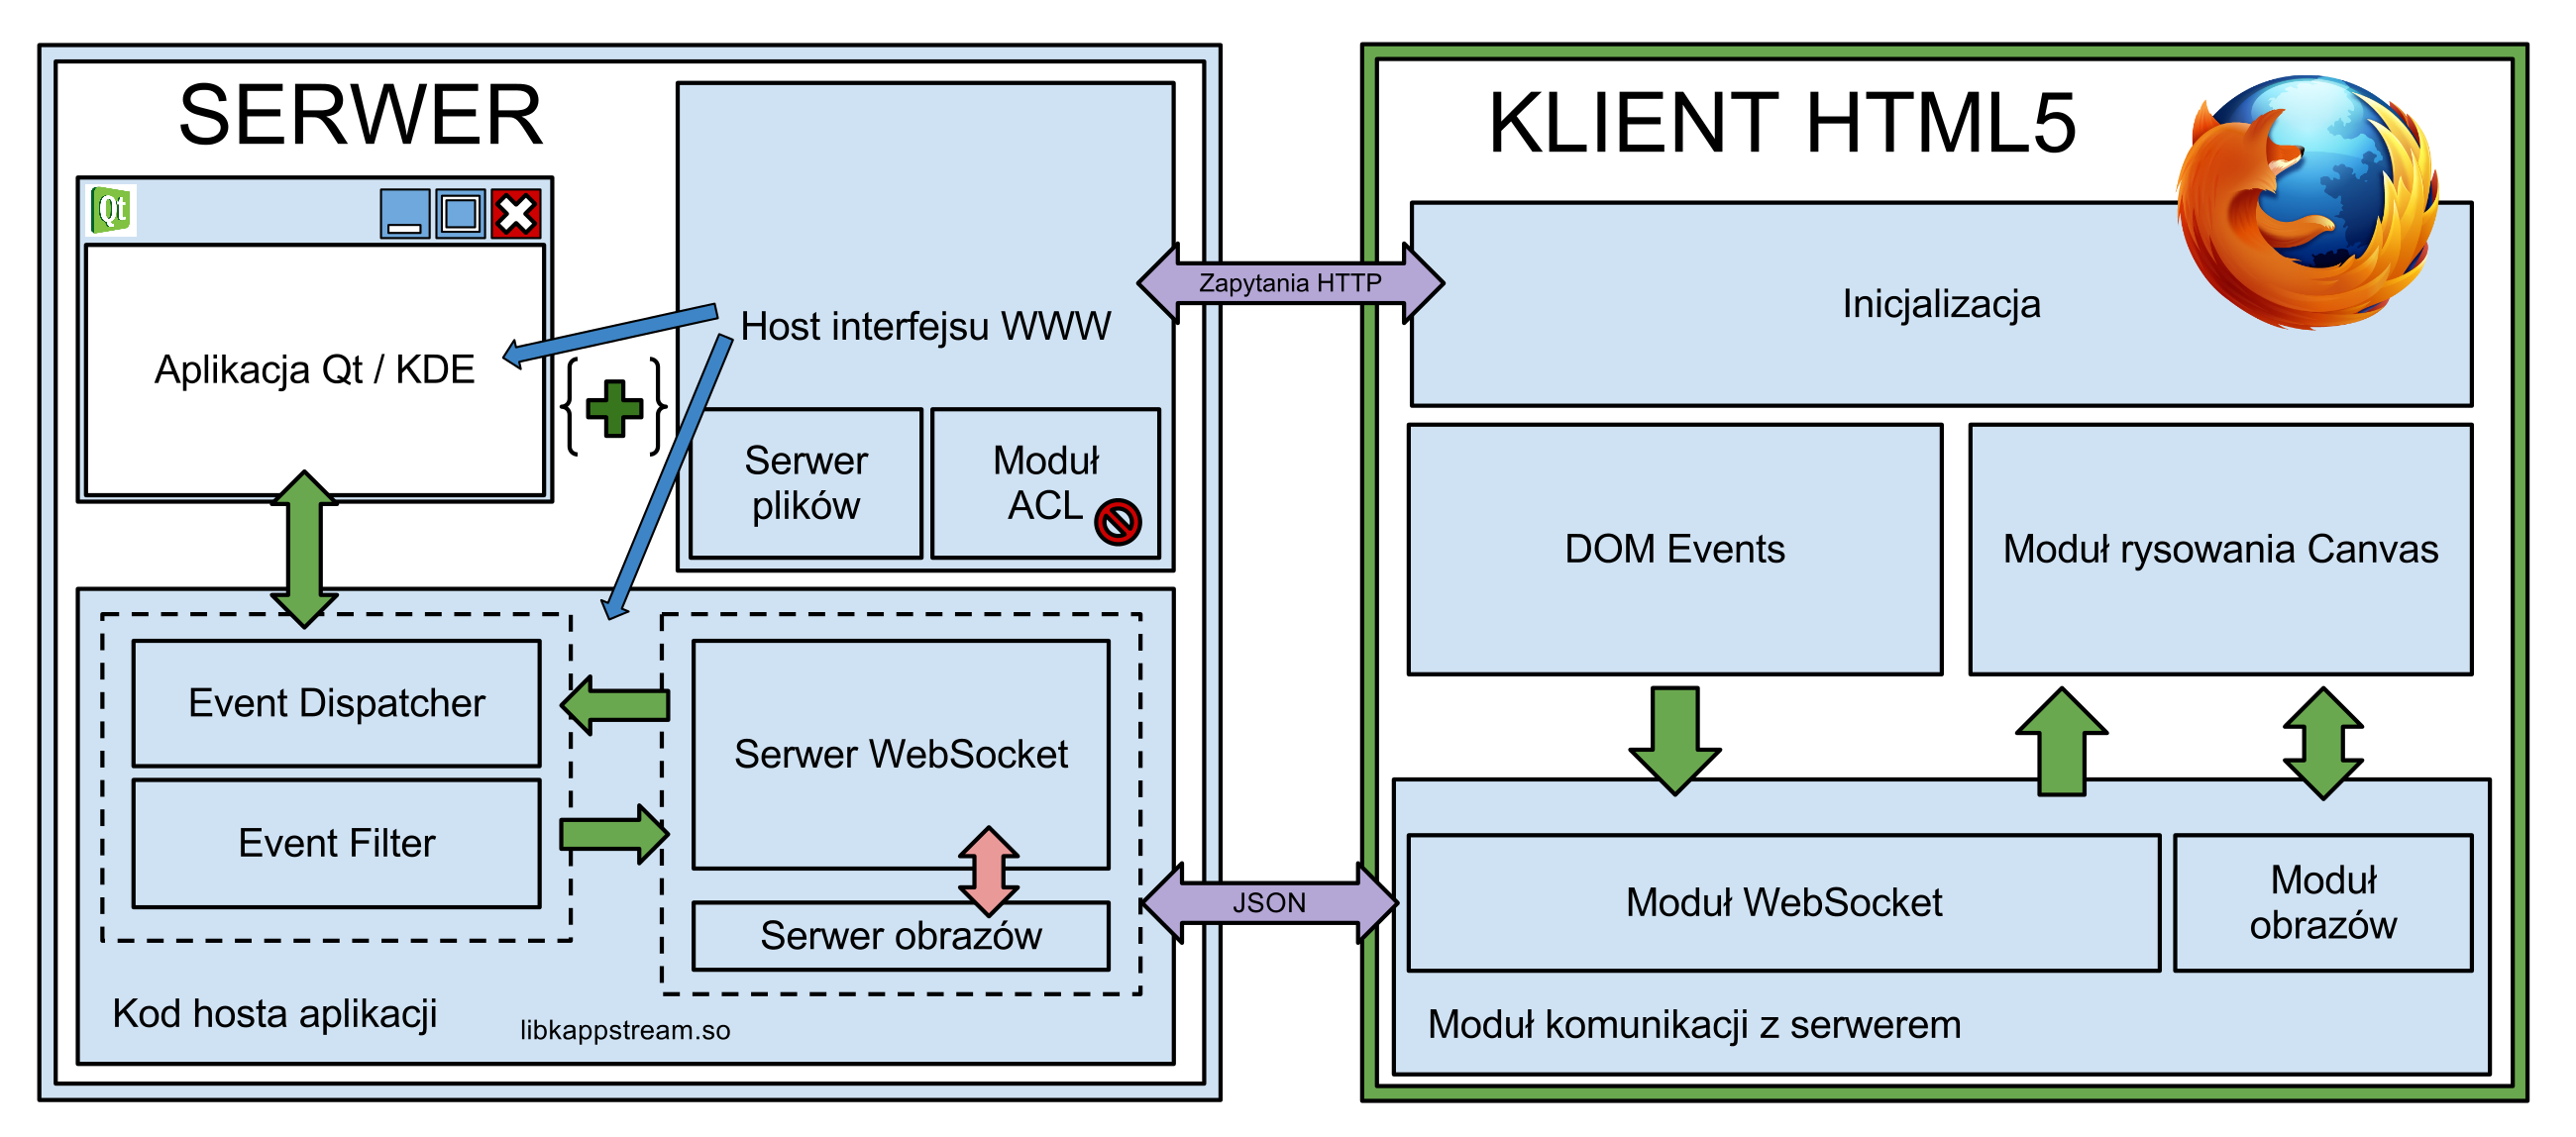
\includegraphics[width=1.0\linewidth]{img/arch}
\caption{Schemat architektury systemu.}
\label{fig:arch}
\end{figure}

\section{Komunikacja między klientem a serwerem}
%Specyfiką problemu jest jego dwuetapowość. W pierwszym etapipe klient inicjuje połączenie jednorazowo wysyłając zapytanie zawierające informacje o aplikacji, którą klient chce uruchomić oraz identyfikatorze klienta. W drugiej kolejności wymagane jest utworzenie kanału komunikacyjnego między klientem a procesem aplikacji. 

Do realizacji tego zadania stworzony został prosty serwer WWW działający w oparciu o protokół \emph{HTTP}. Jego architektura została przedstawiona na rysunku \ref{fig:arch-www}. Jako zasób domyślny udostępnia on listę dostępnych aplikacji, które klient może uruchomić. Lista ta jest w pełni konfigurowalna po stronie serwera. Inicjalizacja połączenia polega na wysłaniu przez klienta identyfikatora wybranej aplikacji. Serwer po pomyślnej weryfikacji przydziela klientowi unikatowy identyfikator sesji, uruchamia proces aplikacji i wysyła klientowi skrypt w języku JavaScript zajmujący się przetwarzaniem po stronie klienta. Każde zapytanie klienta jest weryfikowane za pomocą modułu ACL\footnote{ang. Access Control List}, który sprawdza czy konfiguracja serwera zezwala na uruchamianie żądanych aplikacji. Szczegółowy opis modułu przedstawiono w sekcji \ref{sec:server-security}.

\begin{figure}[H]
\centering
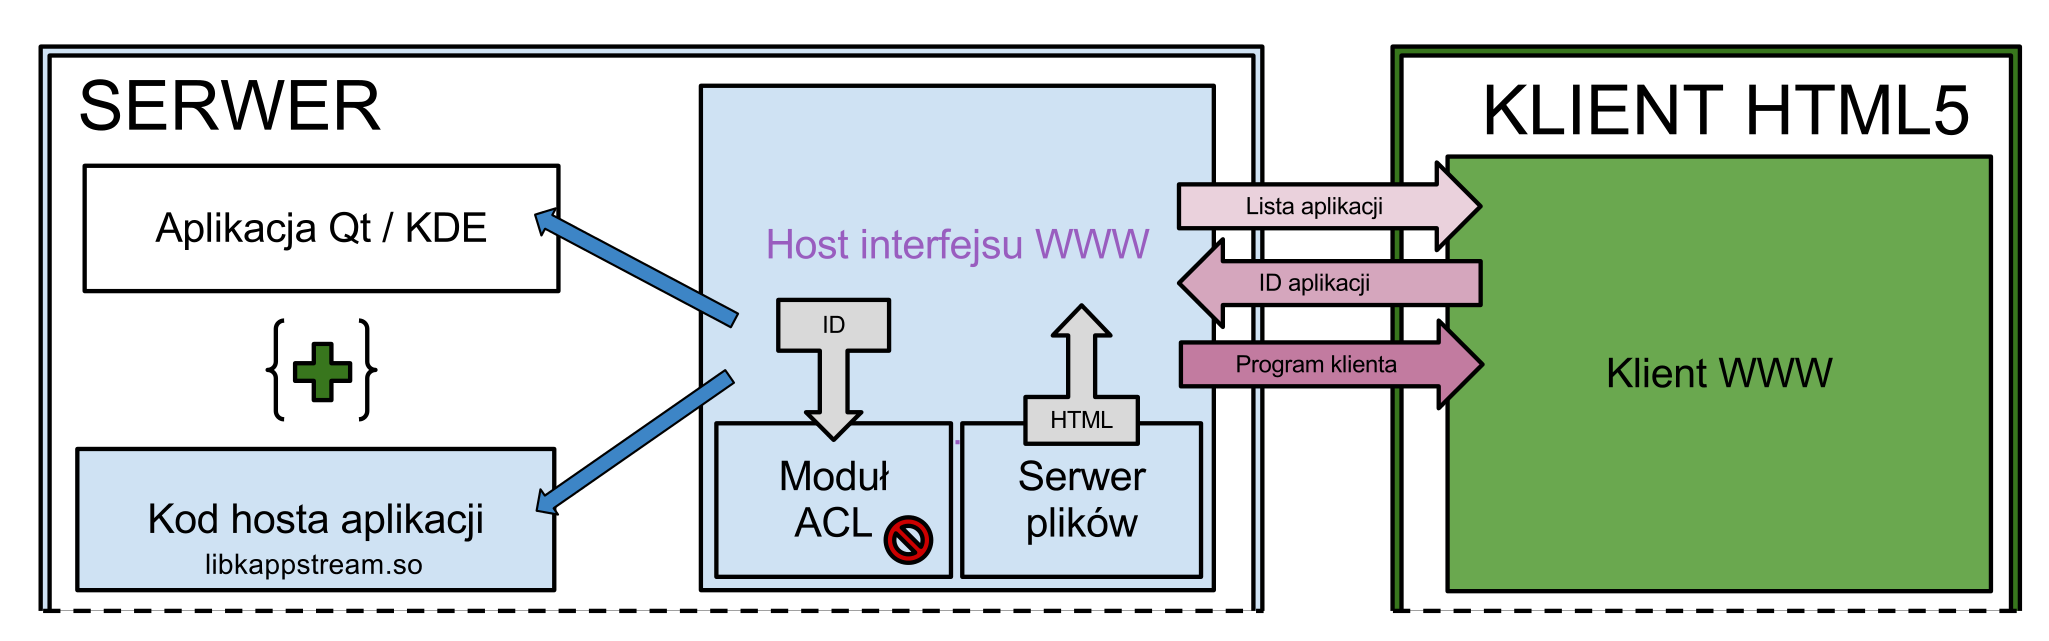
\includegraphics[width=1.0\linewidth]{img/arch-www}
\caption{Schemat komunikacji z serwerem WWW.}
\label{fig:arch-www}
\end{figure}

\section{Komunikacja między klientem a aplikacją}

// TODO: Opis do cz. teoretycznej (pogrubione)

Do rozwiązania tego problemu konieczne jest utworzenie ciągłego kanału komunikacyjnego między klientem a procesem aplikacji, za pomocą którego będzie możliwe przesyłanie informacji o wyglądzie interfejsu aplikacji oraz informowanie aplikacji o zdarzeniach generowanych przez użytkownika po stronie przeglądarki. Jako, że za cel przyjęte zostało założenie o nieingerowaniu bezpośrednio w kod skompilowanych już aplikacji, postawiono na technikę umożliwiającą załadowanie kodu biblioteki dynamicznej do przestrzeni pamięciowej procesu aplikacji tuż przed jego uruchomieniem. Kod ten ma za zadanie utrzymanie połączenia oraz transmisję danych między klientem a aplikacją.

\begin{figure}[H]
\centering
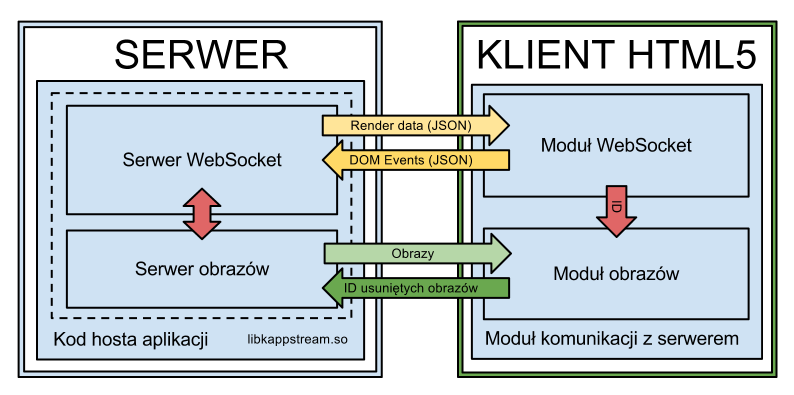
\includegraphics[width=1.0\linewidth]{img/arch-socket}
\caption{Schemat komunikacji z modułem WebSocket.}
\label{fig:arch-socket}
\end{figure}

\section{Uzyskanie informacji o wyglądzie elementów graficznego interfejsu aplikacji}
Każdy element graficznego interfejsu aplikacji (QWidget) jest renderowany w momencie odebrania zdarzenia QPaintEvent z kolejki zdarzeń głównego wątku aplikacji. Dzięki temu istnieje łatwy sposób na uzyskanie informacji o tym kiedy oraz ktory element należy przerenderować aby uaktualnić jego wygląd po stronie klienta. Problemem w dalszyb ciągu pozostaje jednak sposób na uzyskanie informacji o samym wyglądzie. 

Proponowane rozwiązanie polega na zaimplementowaniu abstrakcyjnego urządzenia wyjściowego reprezentującego przeglądarkę WWW po stronie klienta (patrz podrozdział \ref{system_rysowania}). Odpowiednio implementując klasy \emph{QPaintEngine} oraz \emph{QPaintDevice} możliwe staje się uzyskanie szczegółowych informacji dotyczących wygądu widgetów co z kolei umozliwia stworzenie \bf{innowacyjnego} formatu przesyłanych danych. Zamiast przesyłać bitmapy z wyrenderowanym elementem można wysłać informację o kolorach, punktach, liniach i innych podstawowych elementach, które zostaną narysowane na urządzeniu docelowym jakim po stronie klienta jest przeglądarka WWW z obsługą elementów \emph{canvas}.


// TODO Komentarz Co to znaczy innowacyjnego?

\section{Symulacja interakcji użytkownika z interfejsem aplikacji}
Interakcja użytkownika z aplikacją sprowadza się do obsługi następujących zdarzeń:
\begin{enumerate}
  \item ruch myszy nad elementem,
  \item wciśnięcie, zwolnienie oraz dwuklik przycisku myszy,
  \item zmiana położenia kółka myszy,
  \item wciśnięcie oraz zwolnienie klawiszy na klawiaturze,
  \item zmiana rozmiaru okna aplikacji poprzez przeciąganie jego krawędzi,
  \item zamknięcie, minimalizacja lub maksymalizacja okna aplikacji.
\end{enumerate}
Większość z wyżej wymienionych elementów jest obsługiwana jako zdarzenia w języku JavaScript większości dzisiejszych przeglądarek. Proponowane podejście na rozwiązanie tego zagadnienia polega na stworzeniu formatu danych bazując na notacji JSON (JavaScript Object Notation). Dane w tym formacie przesyłane do serwera są następnie poddawane walidacji i konwersji na obiekty zdarzeń biblioteki \emph{Qt}. Zdarzenia takie są następnie przesyłane do kolejki zdarzeń w głównym wątku aplikacji.

Odbiorcą zdarzenia jest obiekt, który na rysunku \ref{fig:arch-hook} został oznaczony jako Event Dispather. Moduł ten jest następnie odpowiedzialny za podjęcie akcji w odpowiedzi na dane zdarzenie, polegających na wywołaniu odpowiednich metod na elemencie interfejsu graficznego aplikacji, który wygenerował dane zdarzenie po stronie przeglądarki bazując na hierarchicznej budowie interfejsu użytkownika.
Wyjątkami są tutaj zdarzenia klawiatury, które nie mają bezpośredniego odbiorcy w momencie ich zaistnienia. Aplikacja na ogół sama decyduje o tym, który element powinien odebrać zdarzenie. Domyślnie jest to widget, który atualnie posiada tzw. focus, a to z kolei zależy od poprzednich zdarzeń oraz logiki samego programu. W celu symulacji podobnego zachowania moduł Event Dispather wybiera element interfejsu bazując na aktualnym stanie aplikacji i wysyła informację o wciśnięciu wirtualnych klawiszy. 

Taka struktura modułu obsługi zdarzeń zapewnia jednolitość działania aplikacji pomiędzy różnymi wersjami biblioteki Qt.

\section{Odtwarzanie aplikacji po stronie klienta}
Aby umożliwić renderowanie elementów po stronie klienta należało utworzyć wspólny format danych bazując na wejściu ze strony biblioteki Qt oraz potrzebnych danych wyjściowych dla obiektu Canvas w języku HTML5. 

Każda komenda rysowania po stronie klienta składa się z podstawowych informacji dotyczących rysowanego obiektu, takich jak: identyfikator, pozycja czy rozmiar, oraz listy prostych elementów z których danych obiekt jest złożony (linie, prostokąty, etc.). Poniżej przedstawiono format pojedyńczej komendy rysowania.


\begin{lstlisting}[language=JavaScript,caption=Komenda renderowania elementu interfejsu]
{
  "command":"draw",
  "widget":{
    "id": 12431,          // Identyfikator
    ["z": 0,]             // Pozycja na stosie obiektow potomnych
    "name":"QLineEdit",   // Nazwa obiektu
    "flags": 0x1029,      // Flagi obiektu (definiuja jego typ 
                          // i wlasciwosci)
    "x": 100,             // Pozycja X
    "y": 120,             // Pozycja Y
    "w": 200,             // Szerokosc
    "h": 150,             // Wysokosc
    "r":{                 // Renderowany obszar elementu
      "x": 0,             // Pozycja obszaru X
      "y": 0,             // Pozycja obszaru Y
      "w": 200,           // Szerokosc obszaru
      "h": 150,           // Wysokosc obszaru
    }
  },
  "render":[]             // Lista elementow do narysowania
}
\end{lstlisting}

Poniżej w kolejności alfabetycznej przedstawiono elementy, z których może być zbudowany każdy obiekt klasy QWidget. Każdy opis zawiera deklarację metody podklasy QPaintEngine wykorzystywanej po stronie serwera, format przesyłanych danych oraz sposób interpretacji tych danych po stronie klienta.

\subsection{Elipsy}
\begin{lstlisting}[language=C++,numbers=none]
virtual void QPaintEngine::drawEllipse( const QRectF & rect );
virtual void QPaintEngine::drawEllipse( const QRect & rect );
\end{lstlisting}
\begin{lstlisting}[language=JavaScript,numbers=none]
{
  "t":"ellipse",
  "x":0.0,       // Pozycja srodka X
  "y":0.0,       // Pozycja srodka Y
  "w":10.0,      // Srednica pozioma
  "h":10.0       // Srednica pionowa
}
\end{lstlisting}

\subsection{Kwadraty}
\begin{lstlisting}[language=C++,numbers=none]
virtual void QPaintEngine::drawRects( const QRectF * rects, 
                                      int rectCount );
virtual void QPaintEngine::drawRects( const QRect * rects, 
                                      int rectCount );
\end{lstlisting}
\begin{lstlisting}[language=JavaScript,numbers=none]
{
  "t":"rect",
  "x":0.0,      // Pozycja lewego-gornego wierzcholka X
  "y":0.0,      // Pozycja lewego-gornego wierzcholka Y
  "w":10.0,     // Szerokosc
  "h":10.0      // Wysokosc
}
\end{lstlisting}

\subsection{Linie}
\begin{lstlisting}[language=C++,numbers=none]
virtual void QPaintEngine::drawLines( const QLineF * lines, 
                                      int lineCount );
virtual void QPaintEngine::drawLines( const QLine * lines, 
                                      int lineCount );
\end{lstlisting}
\begin{lstlisting}[language=JavaScript,numbers=none]
{
  "t":"line",
  "xs":0.0,    // Pozycja startowa X
  "ys":0.0,    // Pozycja startowa Y
  "xe":10.0,   // Pozycja koncowa X
  "ye":10.0    // Pozycja koncowa Y
}
\end{lstlisting}

\subsection{Obrazy}
\begin{lstlisting}[language=C++,numbers=none]
virtual void QPaintEngine::drawImage( const QRectF & rectangle, 
                                      const QImage & image, 
                                      const QRectF & sr, 
                                      Qt::ImageConversionFlags flags = Qt::AutoColor );
virtual void QPaintEngine::drawPixmap( const QRectF & r, 
                                       const QPixmap & pm, 
                                       const QRectF & sr );
virtual void QPaintEngine::drawTiledPixmap( const QRectF & rect, 
                                            const QPixmap & pixmap, 
                                            const QPointF & p );
\end{lstlisting}
\begin{lstlisting}[language=JavaScript,numbers=none]
{
  "t":"image",
  "data":"Ja8SA9c72b71HDj8", // Identyfikator obrazu
  "x":0.0,                   // Pozycja X
  "y":0.0                    // Pozycja Y
}
\end{lstlisting}

Pełna implementacja, natywnie wspierane w \emph{canvas} za pomocą metody drawImage.

\subsection{Wielokąty}
\begin{lstlisting}[language=C++,numbers=none]
virtual void QPaintEngine::drawPolygon( const QPointF * points, 
                                        int pointCount, 
                                        PolygonDrawMode mode );
virtual void QPaintEngine::drawPolygon( const QPoint * points, 
                                        int pointCount, 
                                        PolygonDrawMode mode );
\end{lstlisting}
\begin{lstlisting}[language=JavaScript,numbers=none]
{
  "t":"polygon",
  "mode":0, // 0: QPaintEngine::OddEvenMode
            // 1: QPaintEngine::WindingMode
            // 2: QPaintEngine::ConvexMode
            // 3: QPaintEngine::PolylineMode	
            // http://doc.qt.digia.com/stable/qpaintengine.html#PolygonDrawMode-enum
  "data":   // Lista punktow do polaczenia
    [
      [0.0,0.0],
      [10.0,10.0],
      [123.0,123.0]
    ]
}
\end{lstlisting}

Pełna implementacja, natywnie wspierane w \emph{canvas} za pomocą metod \emph{moveTo}, \emph{lineTo} oraz \emph{closePath}.

\subsection{Punkty}

\begin{lstlisting}[language=C++,numbers=none]
virtual void QPaintEngine::drawPoints( const QPointF * points, 
                                       int pointCount );
virtual void QPaintEngine::drawPoints( const QPoint * points, 
                                       int pointCount );
\end{lstlisting}
\begin{lstlisting}[language=JavaScript,numbers=none]
{
  "t":"points",
  "data":              // Lista punktow
    [
      [0.0,0.0],
      [10.0,10.0],
      [123.0,123.0]
    ]
},
\end{lstlisting}

Pełna implementacja, natywnie wspierane w \emph{canvas}, za pomocą \emph{strokeRect} rysowany jest kwadrat o rozmiarach 1 na 1 piksel.

\subsection{Ścieżki}
\begin{lstlisting}[language=C++,numbers=none]
virtual void QPaintEngine::drawPath( const QPainterPath & path );
\end{lstlisting}
\begin{lstlisting}[language=JavaScript,numbers=none]
{
  "t":"path",
  "data":          // Lista punktow
    [
      ["t":0,"p":[[0,0]]],      // moveTo
      ["t":1,"p":[[10,10]]],    // lineTo
      ["t":2,"p":[[10,10],[100,100]]],  // quadTo
      ["t":2,"p":[[10,10],[100,100],[1000,1000]]],  // cubicTo
    ],
  "fill":0 // 0: Qt::OddEvenFill
           // 1: Qt::WindingFill
           // http://doc.qt.digia.com/stable/qt.html#FillRule-enum
}
\end{lstlisting}

Pełna implementacja, natywnie wspierane w \emph{canvas} za pomocą metod \emph{lineTo}, \emph{lineTo}, \emph{quadraticCurveTo} oraz \emph{bezierCurveTo}.

\subsection{Tekst}
\begin{lstlisting}[language=C++,numbers=none]
virtual void QPaintEngine::drawTextItem( const QPointF & p, 
                                         const QTextItem & textItem );
\end{lstlisting}
\begin{lstlisting}[language=JavaScript,numbers=none]
{
  "t":"text",
  "data":
  {
    "text":"Przykladowy tekst",     // Tekst w kodowaniu UTF8
    "ascent":0,                     // Dystans od linii bazowej do 
                                    // najwyzej polozonego punktu
    "descent":0,                    // Dystans od linii bazowej do 
                                    // najnizej polozonego punktu
    "x":0,                          // Pozycja X
    "y":0,                          // Pozycja Y
    "font":"CSS-format font string" // Informacje o czcionce 
                                    // w formacie CSS
  }
}
\end{lstlisting}

\section{Wewnętrzne przepływy danych w module WebSocket serwera}
Moduł serwera służący do przesyłu danych między aplikacją a klientem złożony jest z dwóch głównych części:
\begin{enumerate}
\item komunikacji z aplikacją,
\item komunikacji z klientem.
\end{enumerate}
Komunikują się one przesyłając dane w formacie JSON. Event Dispather posiada jedno wejście przyjmujące opis zdarzeń zaistniałych po stronie klienta. Event Filter posiada dwa wyjścia, którymi przekazuje dane do serwera WebSocket, który następnie przekazuje je klientowi. Jedno wyjście przekazuje opis graficznych elementów interfejsu. Drugie natomiast obrazy w formacie PNG. Powód dla którego postanowiono oddzielić przesyłąnie obrazów od przesyłania opisu w formasie JSON jest zbyt duży narzut na rozmiar pliku graficznego po konwersji do postaci tekstowej. Serwer WebSocket nie wysyła więc obrazów bezpośrednio do klienta. Przesyła mu jedynie indentyfikator obrazu a same dane są przekazywane do serwera obrazów, który stanowi bufor dla plików graficznych. Bufor ten jest na bieżąco opróżniany w momencie gdy klient zdecyduje się pobrać dany obraz.

\begin{figure}[H]
\centering
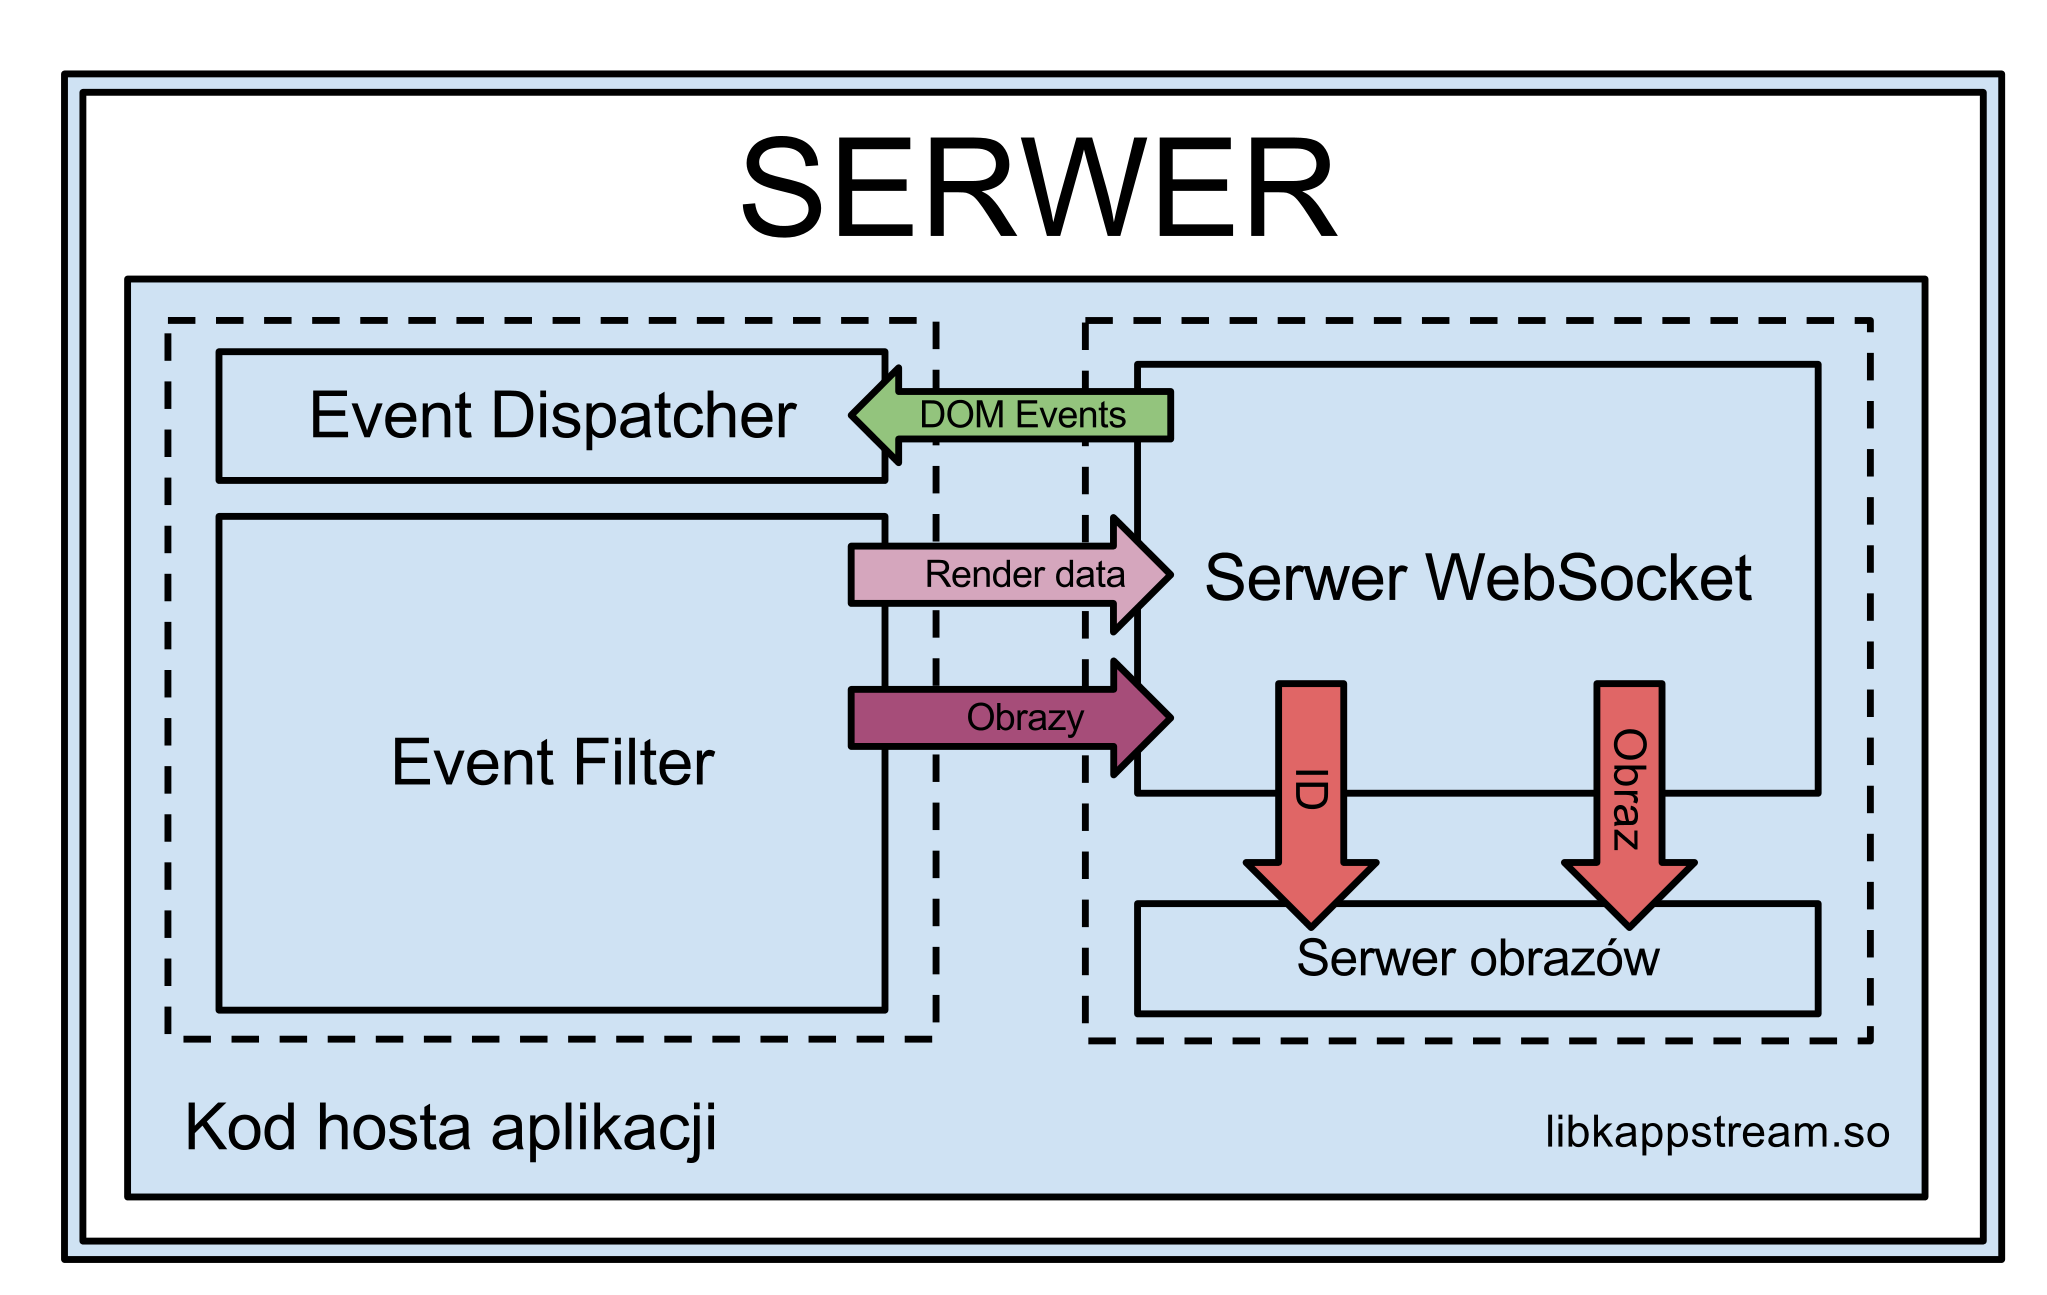
\includegraphics[width=0.8\linewidth]{img/arch-lib}
\caption{Schemat wewnętrznych przepływów danych w module WebSocket.}
\label{fig:arch-lib}
\end{figure}


\section{Zabezpieczenie serwera}
\label{sec:server-security}
Ponieważ jednym z celów projektu było umożliwienie uruchamiania pełnoprawnych aplikacji zainstalowanych na systemie operacyjnym serwera, kluczową staje się możliwość blokowania nieautoryzowanego dostępu do wrażliwych lub potencjalnie niebezpiecznych aplikacji.

W związku z powyższym, stworzono mechanizm list \emph{ACL} (ang. Access Control Lists), który pozwala administratorowi systemu na zdefiniowane, które aplikacje mogą być uruchamiane przez klientów, a w przypadku których zostanie wyświetlony komunikatu o braku dostępu.

Listy kontroli dostępu przechowywane są w pliku konfiguracyjnym serwera w postaci danych w formacie \emph{XML}\footnote{(ang. Extensible Markup Language}. Nazwy aplikacji w postaci komend linii poleceń mogą więc być definiowane ręcznie w dowolnym edytorze tekstowym lub za pomocą pliku wykonywalnego serwera poprzez poniższe argumentów wywołania programu:

\begin{itemize}
\item \emph{accept-all}
spowoduje zniesienie wszystkich wcześniej wprowadzonych obostrzeń i możliwe będzie uruchomienie wszystkich aplikacji zainstalowanych na serwerze,
\item \emph{reject-all}
spowoduje zablokowanie wszystkich zapytań serwera. Komenda ta powinna stanowić pierwszy krok w etapie budowy list dostępu,
\item \emph{accept nazwa-aplikacji} \footnote{Nazwa aplikacji oznacza pełną komendę wiersza poleceń (wraz z możliwymi argumentami), która spowoduje uruchomienie aplikacji. Może to być również ścieżka bezwzględna do pliku wykonywalnego aplikacji.}
spowoduje, że aplikacja o podanej nazwie będzie mogła być uruchamiana przez serwer,
\item \emph{reject nazwa-aplikacji},
komenda blokujaca możliwość uruchamiania aplikacji o podanej nazwie.
\end{itemize}

Serwer, ze względów bezpieczeństwa, od razu po zainstalowaniu domyslnie blokuje wszystkie zapytania klientów i oczekuje się od administratora serwera skonfigurowania list \emph{ACL} według uznania. Zmiana ustawień serwera wymaga jego ponownego uruchomienia.
